\section{Client}

As the client is just going to take care of getting rules for a single sensor
from the central server, and should just apply these to one sensor, the
architecture of the client can be much simpler than the one of the server.

\subsection{Architecture}

The MVC schema for the client would look like this:

\begin{figure}[H]
	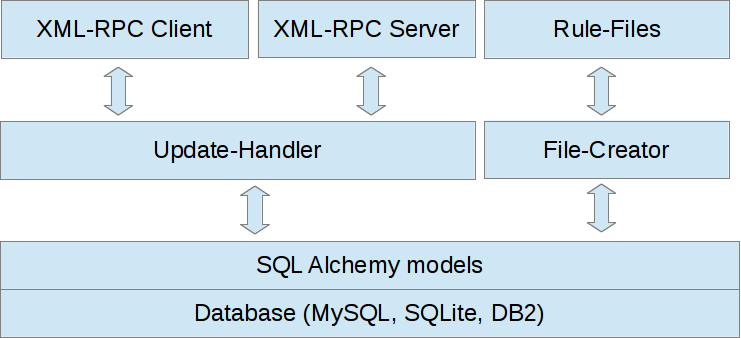
\includegraphics[width=130mm]{./img/Client-MVC.png}
	\caption{Client Architecture}
	\label{client_architecture}
\end{figure}

The update-handler of the client have both a XML-RPC Client and a XML-RPC
Server. The client is used to connect to the central server, to do a
rule-synchronization. The rpc-server is here so that the central server can
connect to it and check that the client is alive, or to order an update of the
rule-sets.

As the client should be as light-weight as possible, and the only thing we would
like to have a framework for is the database-connection, we have decided to not
pull inn Django for the client. Instead we use the database ORM for python
called "SQL-Alchemy".

\subsection{Database}

The database on the client would be significantly simpler than the one on the
server, as we only care about the rules which should be present on a given
sensor.

\begin{figure}[H]
	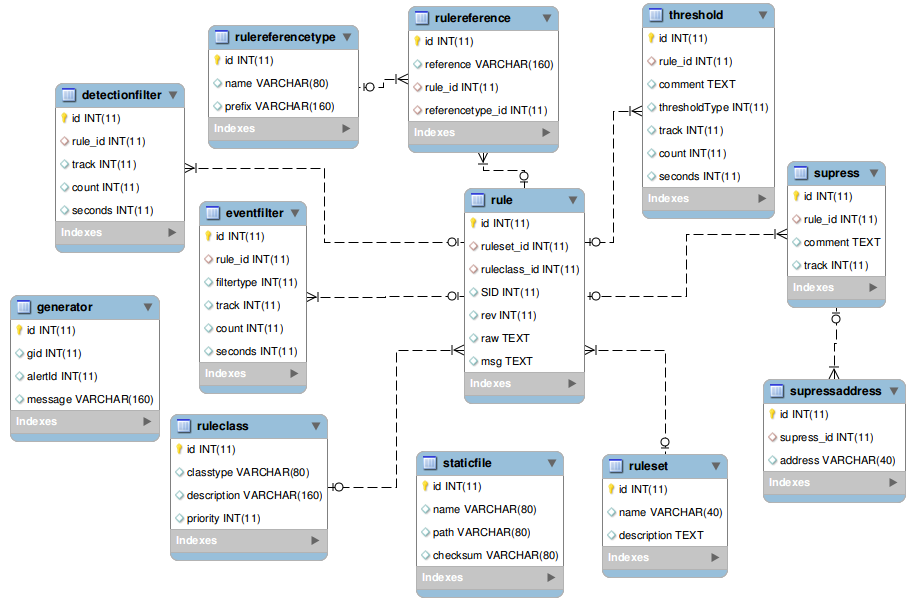
\includegraphics[width=130mm]{./img/Client_Database.png}
	\caption{Client Database}
	\label{client_database}
\end{figure}

The central part of the datastructure is the rule table. This table contains all
the parametres directly related to the rule. In addition we have seperate tables
to all the parametres modifying the rule (like filters), or that is common
between several rules (like rulesets).
